\documentclass[a4paper,11pt]{article}
\usepackage{graphicx, kotex, biblatex, geometry, setspace, amsmath, amsthm} % Required for inserting images
\addbibresource{refs.bib}
\setstretch{1.25}

\theoremstyle{definition}
\newtheorem{definition}{Definition}

\geometry{
 a4paper,
 left=20mm,
 right=20mm,
 top=10mm,
 bottom=15mm
 }
% 이 부분의 값을 조정하여, 상하좌우 공백의 간격을 조절할 수 있습니다. 분량이 많을 경우, 이 부분을 획기적으로 줄이시면 글을 많이 담을 수 있습니다!

\begin{document}
\begin{center}
    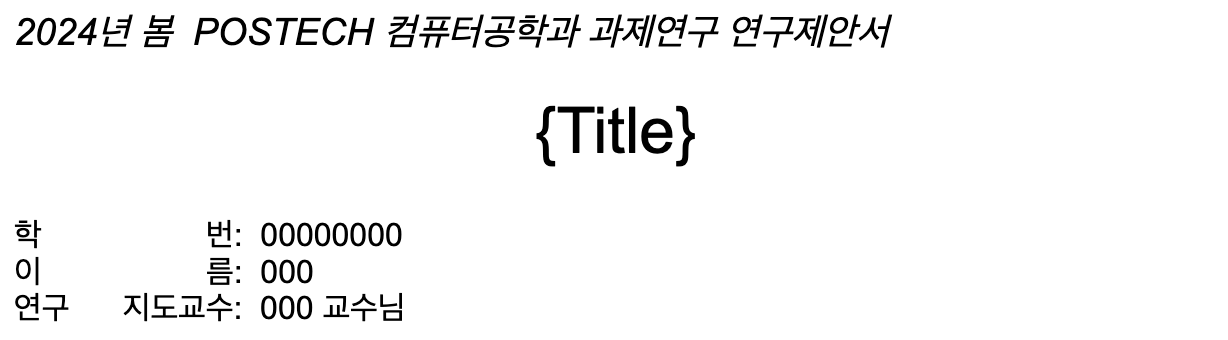
\includegraphics[width=\textwidth]{title.png}
    %이미지는 알아서 캡처한걸로 바꾸시면 됩니다.
\end{center}

% section은 proposal, progress, fianl에 맞게 조정하여 사용하길 바랍니다.

\section{연구 목적(Problem Statement)} % 연구의 주제를 서술하고 그 중요성과 필요성을 설명합니다.
본 연구는 새로운 무언가를 제안합니다. \vspace{2mm} \\ 
어떤 분야에서는 \cite{} 등의 여러 가지 해결책들이 제안되어 왔다. 

\section{연구 배경(Motivation and Background)} % 연구의 배경을 서술하여 계획하는 연구가 가지는 맥락을 밝힙니다. 기존의 연구의 한계와 문제점을 명확하게 서술합니다
\subsection{Subsection1}
subsection을 활용할 수 도 있습니다.
\subsection{Subsection2}
subsection을 활용할 수 도 있습니다.

다음처럼 정의를 작성할 수도 있습니다. 
\begin{definition}$\epsilon$-Indistinguishability (Privacy Leakage)
\begin{align*}
    \left| \ln( \frac{\Pr[\mathcal{M}(D) \in S_\mathcal{M}]}{\Pr[\mathcal{M}(D^{'}) \in S_\mathcal{M}]} ) \right| \leq \epsilon
\end{align*}
\end{definition}

문단에 들여쓰기가 싫다면 \noindent 를 사용하세요.


\paragraph{Paragraph 이름}
subsection의 하위 분야로 Paragraph를 사용할 수 있습니다.

\section{연구 방법 (Research Proposal)} % 문제 해결을 위한 연구 수행 방법을 간략히 서술합니다. 

\section{기대 효과 (Expected Output)} % 연구 결과를 통해 기대할 수 있는 학계 또는 산업계의 파급 효과를 간략히 서술합니다. 

Contribution
\begin{itemize}
    \item 기여1
    \item 기여2
    \item 기여3
\end{itemize}

\section{연구 진행 상황 (Progress Report)}

\section{참고 문헌}
\printbibliography[heading=none]

\section{연구 추진 일정}
\begin{center}
\begin{tabular}{ |c|c| } 
 \hline
 날짜 & 내용 \\
 \hline
?월 ?일 & 연구 제안서 제출 \\
 \hline
\end{tabular}
\end{center}

\section{연구 결과 및 평가(Methodology and Evaluation)}

\section{토론 및 전망 (Discussion and Future work)}

\end{document}
